\documentclass[aspectratio=169]{beamer}

\usepackage{../algpseudocodex}
\usepackage{amssymb}
\usepackage{biblatex}
\usepackage{booktabs}
\usepackage[binary-units]{siunitx}
\usepackage{subcaption}
\usepackage{tikz}

\addbibresource{../refs.bib}

\usetikzlibrary{graphs,graphdrawing}
\usegdlibrary{circular,trees}

\usetheme{metropolis}

\metroset{numbering=fraction,block=fill}
\setbeamertemplate{section in toc}[sections numbered]

\author{Leonard Techel}
\title{Low-Connectivity State Space Exploration using Swarm Model Checking on the GPU}
\date{October 7, 2021}

\begin{document}

\maketitle

\begin{frame}{Table of Contents}
    \tableofcontents
\end{frame}

\section{Motivation}

\begin{frame}{Motivation 1/2: Waypoints Benchmark Model}
    \begin{itemize}
        \item Current state: Represented by a \SI{32}{\bit} integer
        \item Eight concurrent processes, each in control of four bits
        \item Each process toggles one random bit on successor generation
        \item \textbf{Goal:} Find 100 random uniform distributed \SI{32}{\bit} integers (Waypoints)
    \end{itemize}

    \medskip

    \begin{figure}
        \only<1>{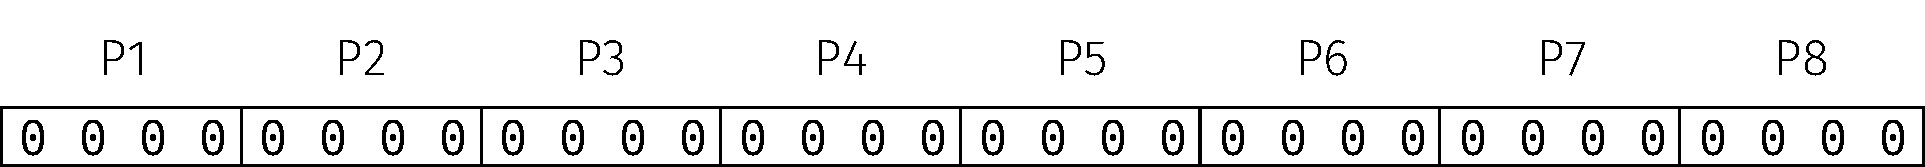
\includegraphics[width=\textwidth]{../figures/waypoints-model.pdf}}%
        \only<2>{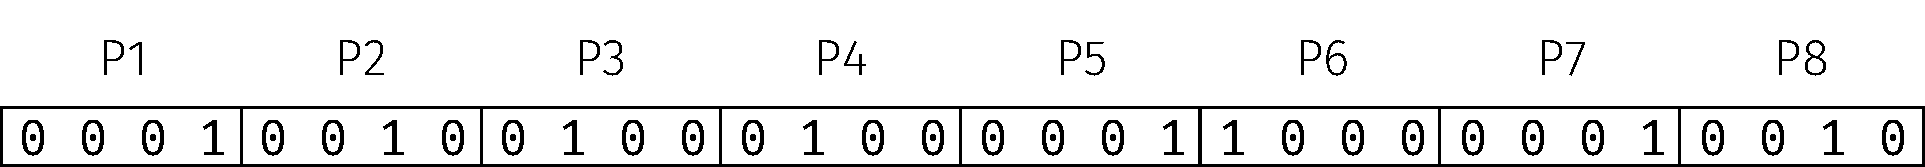
\includegraphics[width=\textwidth]{../figures/waypoints-model-1.pdf}}%
        \only<3>{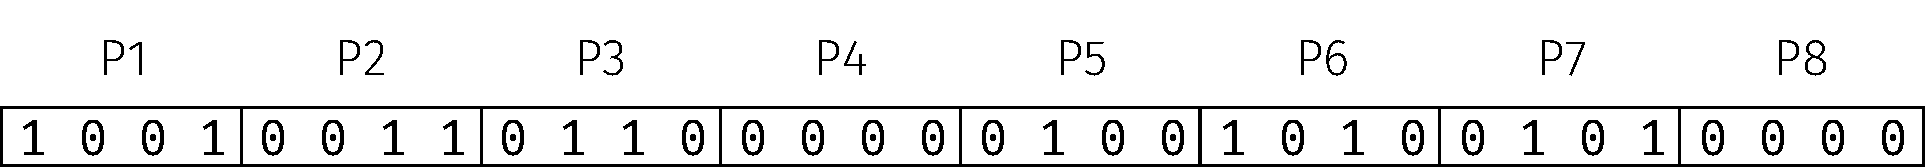
\includegraphics[width=\textwidth]{../figures/waypoints-model-2.pdf}}%
        \vspace{\baselineskip}
        \caption{Waypoints model state}
        \label{fig:waypoints-model}
    \end{figure}
\end{frame}

\begin{frame}{Motivation 2/2: Observations}
    \begin{itemize}
        \item \textbf{Model Checking:} Verify whether a transition system satisfies a specification
              \medskip
        \item We have $2^{32} = \left(2^4\right)^{\boldsymbol{8}} = \num{4294967296}$ states to check
        \item \textbf{Problem:} State Space Explosion
        \item Exhaustive verification cannot be completed in reasonable time
        \item Storing all states in memory takes up $2^{32} \cdot \SI{32}{\bit} = \SI{17}{\giga\byte}$
        \item What can we do?
    \end{itemize}
\end{frame}

\section{Concepts: Swarm Verification, Grapple Framework, Low-Connectivity Models}

\begin{frame}{Swarm Verification 1/2}
    From the paper \emph{Swarm Verification} by G. J. Holzmann et al. \cite{Holzmann2008.Swarm-Verification}
    \begin{itemize}
        \item Approach on explicit-state model checking
        \item \textbf{Idea:} Split state space exploration into small, independent verification tests (VTs)
        \item Each VT only covers a subset of the state space
        \item \textbf{Result:} VTs can be massively parallelized, for example on the GPU
        \item How is the state space exploration split up?
    \end{itemize}
\end{frame}

\begin{frame}{Swarm Verification 2/2: Diversification Techniques}
    \begin{columns}
        \begin{column}{.5\textwidth}
            Diversification techniques:

            \begin{itemize}
                \item \textbf{State pruning using hash collisions}
                \item Reversing search order
                \item Randomizing order of nondeterministic choice
                \item \dots
            \end{itemize}

            How to implement Swarm Verification on the GPU?
        \end{column}
        \begin{column}{.5\textwidth}
            \begin{figure}
                \begin{subfigure}[b]{.49\textwidth}
                    \resizebox{\textwidth}{!}{
                        \begin{tikzpicture}[nodes={draw, circle}]
                            \graph [tree layout, missing nodes get space] {
                                A [fill=lightgray];
                                B [fill=lightgray];
                                D [fill=lightgray];
                                E [fill=lightgray];
                                F [fill=lightgray];
                                I [fill=lightgray];
                                J [fill=lightgray];

                                A -- B [second];
                                A -- C;
                                A -- D;

                                B -- E;
                                B -- F;

                                C -- F;
                                C -- G;
                                C -- H;

                                D -- I;

                                F -- J;

                                H -- K;
                                H -- L;
                            };
                        \end{tikzpicture}
                    }
                    \subcaption*{Collision: \{B, C\}}
                \end{subfigure}
                \begin{subfigure}[b]{.49\textwidth}
                    \resizebox{\textwidth}{!}{
                        \begin{tikzpicture}[nodes={draw, circle}]
                            \graph [tree layout, missing nodes get space] {
                                A [fill=lightgray];
                                B [fill=lightgray];
                                C [fill=lightgray];
                                D [fill=lightgray];
                                E [fill=lightgray];
                                G [fill=lightgray];
                                H [fill=lightgray];
                                I [fill=lightgray];
                                K [fill=lightgray];
                                L [fill=lightgray];

                                A -- B;
                                A -- C;
                                A -- D;

                                B -- E;
                                B -- F;

                                C -- F;
                                C -- G;
                                C -- H;

                                D -- I;

                                F -- J;

                                H -- K;
                                H -- L;
                            };
                        \end{tikzpicture}
                    }
                    \subcaption*{Collision: \{E, F\}}
                \end{subfigure}
                \caption{State pruning using hash collisions}
                \label{figure:hash-collision-state-pruning}
            \end{figure}

        \end{column}
    \end{columns}
\end{frame}

\begin{frame}{Grapple Model Checking Framework}
    From the paper \emph{Swarm model checking on the GPU} by R. DeFrancisco et al. \cite{DeFrancisco2020.Grapple}

    \begin{itemize}
        \item A framework for parallel Swarm Verification model checking on the GPU using CUDA
        \item Why GPUs? — GPUs are massively parallel, widely available and cheap
        \item Each VT executes a parallel breadth-first search
    \end{itemize}

    What are the limitations?
\end{frame}

\begin{frame}{Low-Connectivity Models 1/2: Definition}
    \begin{columns}
        \begin{column}{.6\textwidth}
            A model has \emph{low connectivity} if at least one of the following properties is satisfied:
            \begin{itemize}
                \item \textbf{Generally Linear}: The average \# of edges per state is close to 2: One inbound, one outbound
                \item \textbf{Bottleneck Structures}: A single state or group of states other than the initial state that needs to be passed to reach most of the state space
            \end{itemize}
        \end{column}
        \begin{column}{.4\textwidth}
            \begin{figure}
                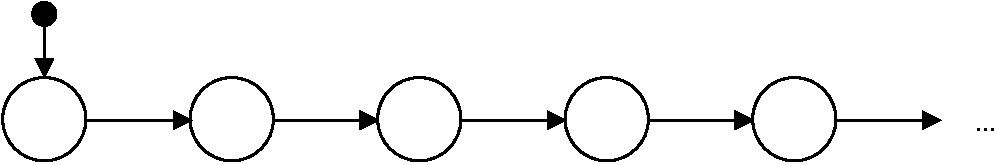
\includegraphics[width=.8\textwidth]{../figures/lc-ex-generally-linear}
                \caption{Example of a generally linear graph}
            \end{figure}
            \begin{figure}
                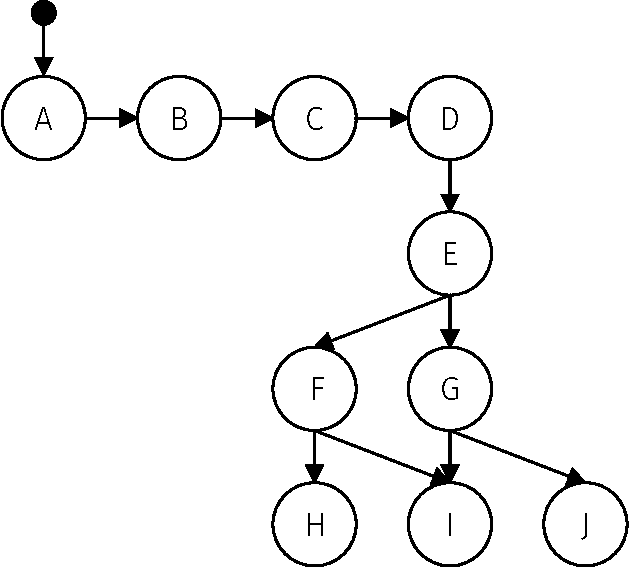
\includegraphics[width=.6\textwidth]{../figures/lc-ex-bottleneck}
                \caption{Example of a bottleneck structure}
            \end{figure}
        \end{column}
    \end{columns}
\end{frame}

\begin{frame}{Low-Connectivity Models 2/2: What to do?}
    \begin{itemize}
        \item According to the paper, coverage slows down: Less unique states visited
        \item Questions proposed in the intermediate presentation:
              \begin{enumerate}
                  \item How can we (automatically) classify a model as low-connectivity?
                  \item How can we improve the state space exploration of such models?
              \end{enumerate}
        \item How can we see the effect? $\rightarrow$ Count unique states visited
    \end{itemize}
\end{frame}

\section{Contributions: Estimating Unique States Visited, Start Overs}

\begin{frame}{Estimating Unique States Visited 1/2}
    \begin{itemize}
        \item Verification Tests may overlap in covered state space
        \item \textbf{Unique States Visited:} Number of unique states visited across all VTs
        \item \textbf{Total States Visited:} Number of states visited by all VTs, including duplicates
    \end{itemize}
\end{frame}

\begin{frame}{Estimating Unique States Visited 2/2}
    \begin{itemize}
        \item<1-> \textbf{Goal:} Observe a swarm's progress in state space coverage

              \begin{itemize}
                  \item How close are we to \SI{100}{\percent} state space coverage?
                  \item How does the exploration of low-connectivity models perform?
              \end{itemize}

        \item<2-> \textbf{Challenge:} Distributed counting of distinct states across all VTs

              \begin{itemize}
                  \item VTs are independent of each other
                  \item VTs may overlap in explored state space
                  \item Each VT visits up to $2^{18}$ states, we have >\num{100000} VTs
              \end{itemize}

        \item<3-> \textbf{Approach:} Probabilistic Cardinality Estimation using HyperLogLog++

              \begin{itemize}
                  \item Estimation with fixed error
                  \item Example: Estimate cardinalities $>10^9$ with a standard error of \SI{2}{\percent} using \SI{1.5}{\kilo\byte} of memory
              \end{itemize}
    \end{itemize}
\end{frame}

\begin{frame}{Start Overs 1/2}
    \begin{itemize}
        \item \textbf{Observation:} All VTs start at the initial state and terminate after ~$2^{18}=\num{262144}$ states due to a full hash table
        \item \textbf{Challenge:} How can we reach deeper states?
        \item \textbf{Approach:} Start Overs as an extension to the Grapple breadth-first search
    \end{itemize}
\end{frame}

\begin{frame}{Start Overs 2/2}
    \begin{itemize}
        \item Self-Contained within a VT
        \item Keep the last few visited states
        \item When the VT's search terminates, use last visited states as new initial states
        \item \textbf{Result:} We can use an even smaller hash table by adding start overs
    \end{itemize}

    Do start overs increase the state space coverage?
\end{frame}

\section{Experimental Results}

 {%
  \setbeamertemplate{frame footer}{HT: Hash table size, as a power of two. SO: Number of start overs}
  \begin{frame}{Start Overs on Waypoints and Low-Connectivity Models 1/2}
      \begin{figure}
          \begin{subfigure}[b]{.49\textwidth}
              \centering
              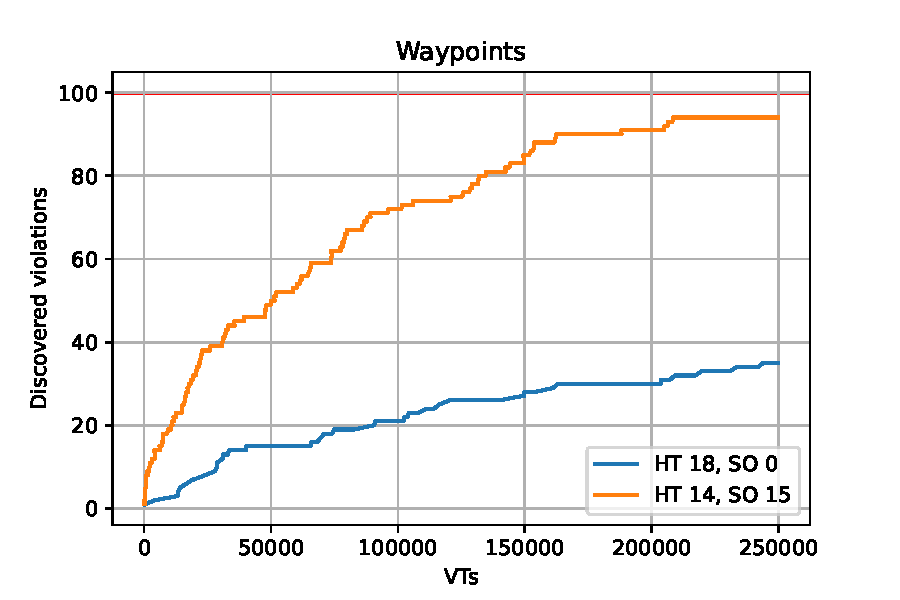
\includegraphics[width=\textwidth]{../../evaluation/output-assets/EXP-04-start-overs-1.pdf}
              \subcaption{Comparison of discovered waypoints}
              \label{fig:evaluation:EXP-04:1}
          \end{subfigure}
          \begin{subfigure}[b]{.49\textwidth}
              \centering
              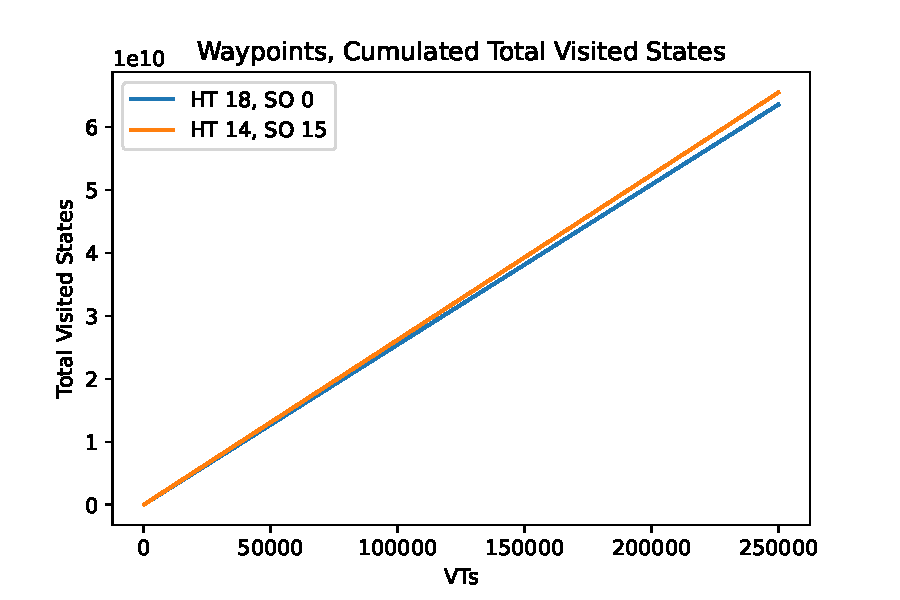
\includegraphics[width=\textwidth]{../../evaluation/output-assets/EXP-04-start-overs-3.pdf}
              \subcaption{Comparison of total visited states}
              \label{fig:evaluation:EXP-04:2}
          \end{subfigure}
          \caption{State space exploration with start overs. \num{250000} VTs}
          \label{fig:evaluation:EXP-04}
      \end{figure}
  \end{frame}

  \begin{frame}{Start Overs on Waypoints and Low-Connectivity Models 2/2}
      \begin{figure}
          \begin{subfigure}[b]{.49\textwidth}
              \centering
              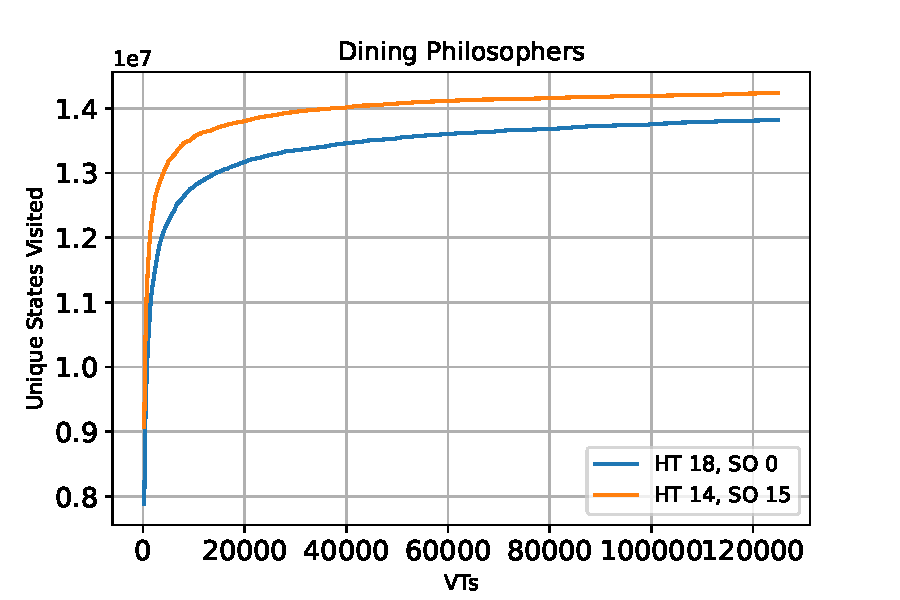
\includegraphics[width=\textwidth]{../../evaluation/output-assets/EXP-13-start-overs-low-connectivity-1.pdf}
              \label{fig:evaluation:EXP-13:1}
          \end{subfigure}
          \begin{subfigure}[b]{.49\textwidth}
              \centering
              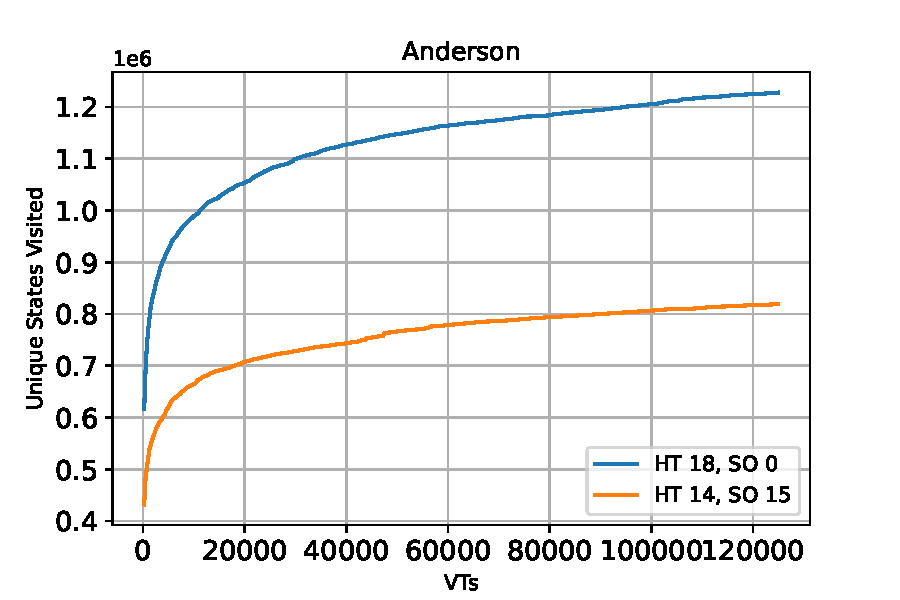
\includegraphics[width=\textwidth]{../../evaluation/output-assets/EXP-13-start-overs-low-connectivity-2.pdf}
              \label{fig:evaluation:EXP-13:2}
          \end{subfigure}
          \caption{Start over strategy on low-connectivity models. \num{125000} VTs}
          \label{fig:evaluation:EXP-13}
      \end{figure}
  \end{frame}
 }

\begin{frame}{Unique and Total States Visited on Low-Connectivity Models}
    \begin{columns}
        \begin{column}{.5\textwidth}
            \begin{figure}
                \centering
                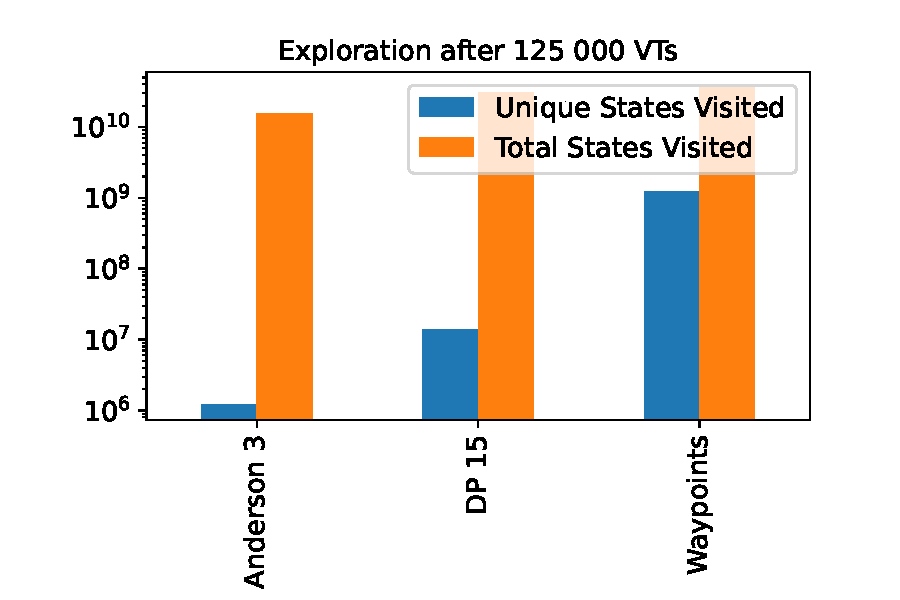
\includegraphics[width=\textwidth]{../../evaluation/output-assets/EXP-12-model-comparison-5.pdf}
                \caption{Exploration of low-connectivity models}
                \label{fig:evaluation:EXP-12}
            \end{figure}
        \end{column}
        \begin{column}{.5\textwidth}
            \begin{itemize}
                \item \textbf{Question:} Do Low-Connectivity models behave differently in terms of USV and TSV?
                \item \textbf{Logarithmic scale!}
                \item Anderson 3: Less than half the total visited states as the waypoints model
                \item Both low-connectivity models: Unique State Hit-Rate <\SI{0.1}{\percent}
            \end{itemize}
        \end{column}
    \end{columns}
\end{frame}

\begin{frame}{BFS Frontiers 1/4}
    \begin{itemize}
        \item<1-> Breadth-first search: Produces \emph{frontiers}
        \item<1-> Current frontier: Deepest states found until now
        \item<1-> Next frontier: Successors of current frontier that are not visited before
        \item<2-> \textbf{Idea:} For each frontier: Count \emph{visited} (= not seen before) and \emph{failed} (= already seen) states
        \item<2-> \textbf{Expectation:} Visited states quickly build up from the single initial state, then decay due to the hash table filling up
    \end{itemize}
\end{frame}

{%
\setbeamertemplate{frame footer}{visited: not seen before. failed: already seen}
\begin{frame}{BFS Frontiers 2/4: Waypoints model}
    \begin{figure}
        \begin{subfigure}[b]{.49\textwidth}
            \centering
            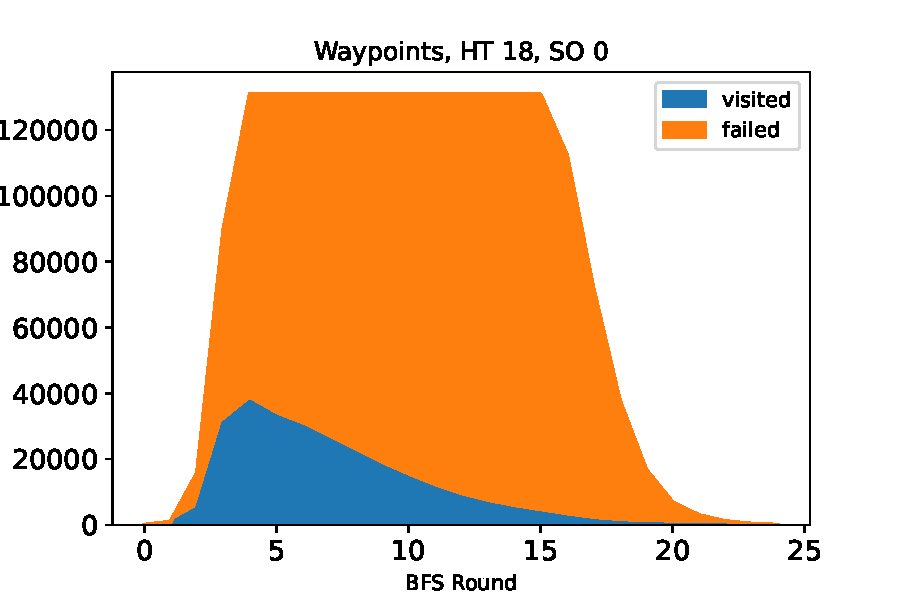
\includegraphics[width=\textwidth]{../../evaluation/output-assets/EXP-11-bfs-frontiers-1.pdf}
            \label{fig:evaluation:EXP-11:1}
        \end{subfigure}
        \begin{subfigure}[b]{.49\textwidth}
            \centering
            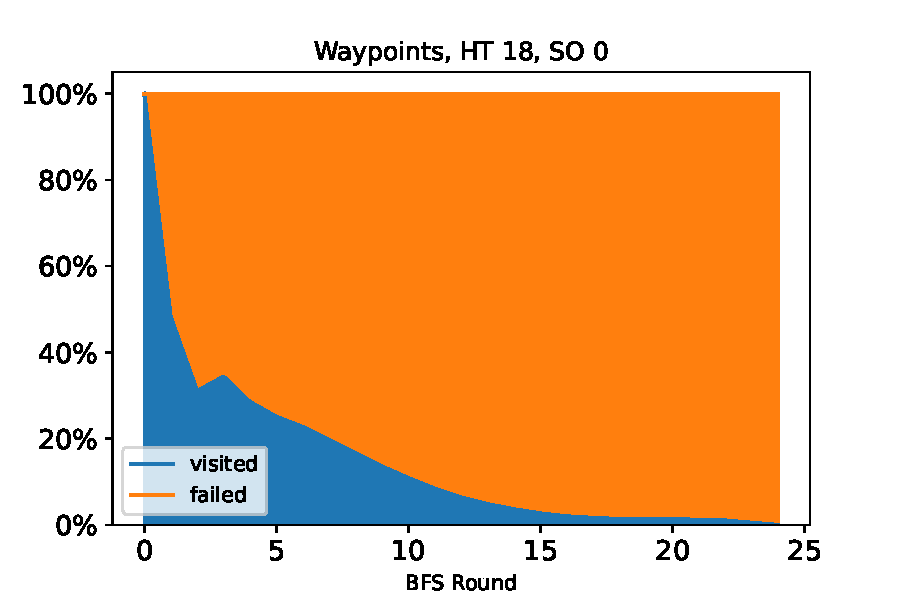
\includegraphics[width=\textwidth]{../../evaluation/output-assets/EXP-11-bfs-frontiers-5.pdf}
            \label{fig:evaluation:EXP-11:5}
        \end{subfigure}
        \caption{BFS frontier visualization of the waypoints model}
        \label{fig:evaluation:EXP-11-1}
    \end{figure}
\end{frame}

\begin{frame}{BFS Frontiers 3/4: Dining Philosophers}
    \begin{figure}
        \begin{subfigure}[b]{.49\textwidth}
            \centering
            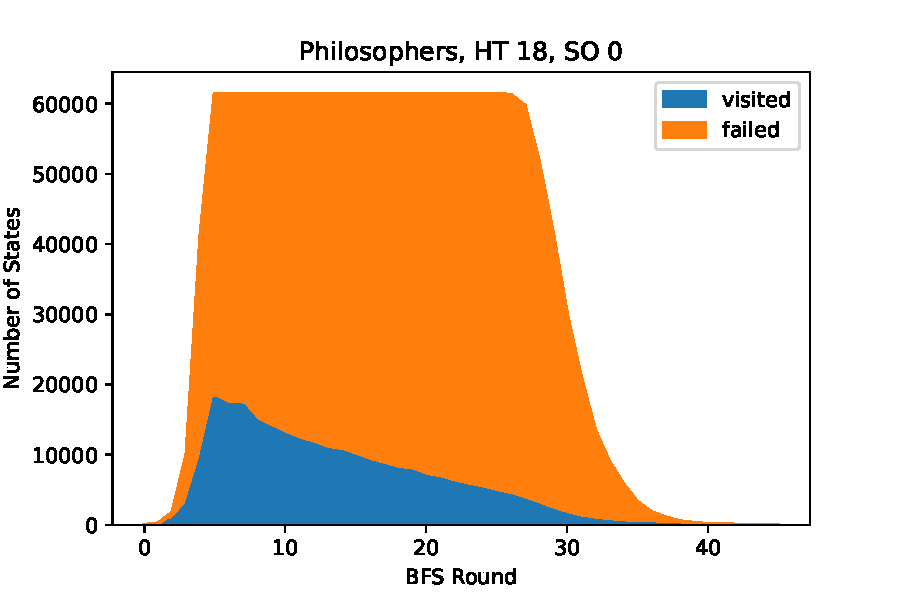
\includegraphics[width=\textwidth]{../../evaluation/output-assets/EXP-11-bfs-frontiers-2.pdf}
            \label{fig:evaluation:EXP-11:2}
        \end{subfigure}
        \begin{subfigure}[b]{.49\textwidth}
            \centering
            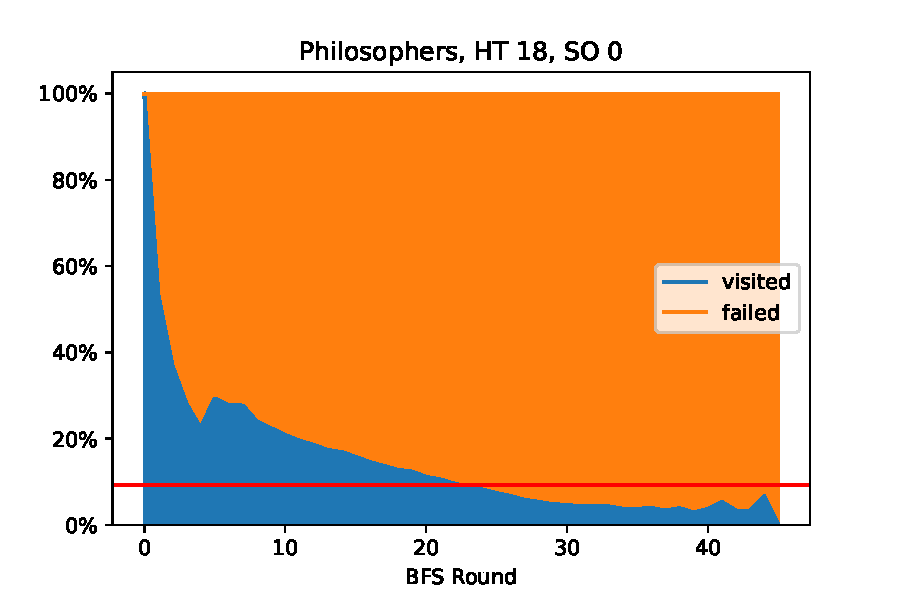
\includegraphics[width=\textwidth]{../../evaluation/output-assets/EXP-11-bfs-frontiers-6.pdf}
            \label{fig:evaluation:EXP-11:6}
        \end{subfigure}
        \caption{BFS frontier visualization of the dining philosophers model}
        \label{fig:evaluation:EXP-11-2}
    \end{figure}
\end{frame}

\begin{frame}{BFS Frontiers 4/4: Anderson model}
    \begin{figure}
        \begin{subfigure}[b]{.49\textwidth}
            \centering
            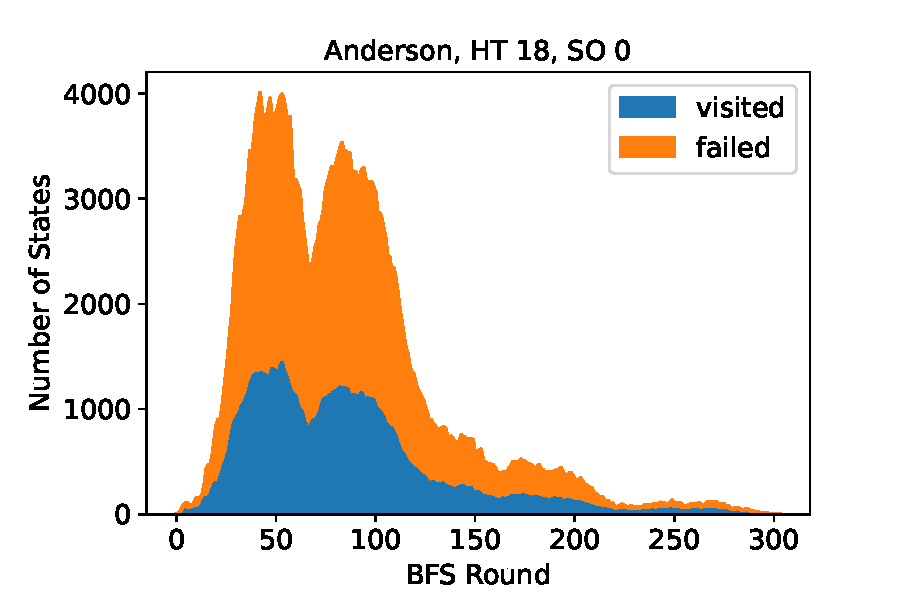
\includegraphics[width=\textwidth]{../../evaluation/output-assets/EXP-11-bfs-frontiers-3.pdf}
            \label{fig:evaluation:EXP-11:3}
        \end{subfigure}
        \begin{subfigure}[b]{.49\textwidth}
            \centering
            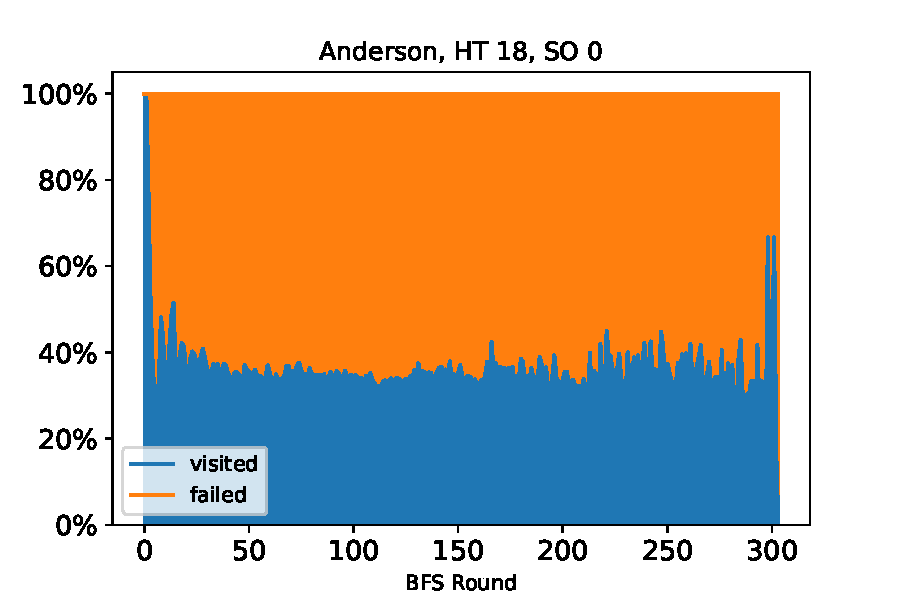
\includegraphics[width=\textwidth]{../../evaluation/output-assets/EXP-11-bfs-frontiers-7.pdf}
            \label{fig:evaluation:EXP-11:7}
        \end{subfigure}
        \caption{BFS frontier visualization of the Anderson 3 model}
        \label{fig:evaluation:EXP-11-3}
    \end{figure}
\end{frame}
}

\section{Conclusions}

\begin{frame}{Conclusions}
    \begin{itemize}
        \item Successfully implemented a Grapple swarm model checker
        \item Successfully estimated unique states visited
        \item Experiments showed promising characteristics on low-connectivity models
        \item One notable exception: Anderson model
    \end{itemize}

    \bigskip

    Thesis, Model Checker, and Experiments: \textbf{\href{https://github.com/barnslig/bachelor-thesis}{github.com/barnslig/bachelor-thesis}}
\end{frame}

\appendix

\begin{frame}{References} % [allowframebreaks]
    \printbibliography[heading=none]
\end{frame}

\end{document}
